Après vous avoir introduit le contexte du projet, nous allons maintenant vous expliquer comment nous avons fait pour implémenter le crypto-système RSA sur un firmware customisé de la ChipWhisperer.

\subsection{Introduction}
Dans cette section, nous abordons l'implémentation du crypto-système RSA sur un firmware personnalisé de la ChipWhisperer. Après avoir établi le contexte du projet, nous décrivons en détail notre démarche pour mettre en œuvre le RSA sur des nombres de 32 bits, en nous appuyant sur les capacités natives du crypto-processeur de la plateforme. Nous explorons les différentes étapes nécessaires à cette implémentation, de la génération des clés à l'exécution des opérations de chiffrement et de déchiffrement, en passant par les algorithmes essentiels tels que l'exponentiation modulaire et le calcul de l'inverse modulaire. Par la suite, nous discutons des défis rencontrés lors de la transition vers une implémentation plus réaliste du RSA, conformément aux normes de sécurité établies par l'ANSSI. Enfin, nous examinons l'approche adoptée pour représenter et manipuler des nombres de grande taille (> 32 bits) dans un environnement embarqué limité, ainsi que les difficultés persistantes rencontrées dans l'implémentation des opérations de réduction modulaire.

\subsection{Implémentation sur 32 bits}
Dans un premier temps, nous avons décidé d'implémenter le RSA sur des petits nombres de taille supportés nativement par le crypto-processeur. Ce dernier utilise une architecture de 32 bits, cela signifie que lorsqu'on stock un nombre dessus, ce nombre ne peut être que de 32 bits maximum (de $0$ à $2^{32} - 1$, pour des entiers positifs). Nous allons donc commencer par implémenter le RSA sur des nombres de 32 bits afin de pouvoir utiliser les opérations usuelles : addition, multiplication, réduction modulaire, ...\\

Comme nous l'avons vu dans la section précédente, pour implémenter le RSA, nous avons besoin de savoir trois choses différentes :
\begin{enumerate}
	\item Générer des clés de chiffrement/déchiffrement ;
	\item Chiffrer un message $m$, sur 32 bits $m < 2^{32}$;
	\item Déchiffrer un chiffré $c$, sur 32 bits $c < 2^{32}$.
\end{enumerate}
\medskip
Les algorithmes nécessaire pour effectuer ces opérations sont : la génération de nombres premiers aléatoire afin de déterminer $p$ et $q$, le calcul d'inverse modulaire pour déterminer la clé privée $d$ tel que $ed \equiv 1 [n]$ et l'exponentiation modulaire afin de chiffrer et déchiffrer, cf. équation (\ref{eq:chiffrement}) et (\ref{eq:dechiffrement}).\\

Nous avons écrit le pseudo-code des ces deux algorithmes essentiels (cf. Algorithme \ref{alg:expomod} et \ref{alg:invmod}), pour ce qui est de leur implémentation en C dans le firmware de la ChipWhisperer, vous pouvez les retrouver dans l'archive finale du projet.

\medskip
\begin{algorithm}[p]
\SetAlgoLined
\KwIn{base, exponent, modulus}
\KwOut{result}
$result \leftarrow 1$\;
$base \leftarrow base \mod modulus$\;
\While{$exponent > 0$}{
  \If{$exponent$ est impair}{
    $result \leftarrow (result \times base) \mod modulus$\;
  }
  $exponent \leftarrow exponent \div 2$\;
  $base \leftarrow (base \times base) \mod modulus$\;
}
\KwRet{$result$}\;
\caption{Pseudo-code de l'exponentiation modulaire}
\label{alg:expomod}
\end{algorithm}
\medskip

\begin{algorithm}[p]
\SetAlgoLined
\KwIn{a, m}
\KwOut{inverse modulaire}
$m0 \leftarrow m$\;
$y \leftarrow 0$\;
$x \leftarrow 1$\;
\If{$m = 1$}{
  \KwRet{$0$}\;
}
\While{$a > 1$}{
  $q \leftarrow a \div m$\;
  $t \leftarrow m$\;
  $m \leftarrow a \mod m$\;
  $a \leftarrow t$\;
  $t \leftarrow y$\;
  $y \leftarrow x - q \times y$\;
  $x \leftarrow t$\;
}
\If{$x < 0$}{
  $x \leftarrow x + m0$\;
}
\KwRet{$x$}\;
\caption{Pseudo-code de l'inverse modulaire}
\label{alg:invmod}
\end{algorithm}

Afin d'illustrer la différence de complexité entre les deux algorithmes d'exponentiation binaire : le naif et le rapide, vous pouvez retrouver sur la Figure \ref{fig:diff_complexite} le graphe du nombres d'opération par rapport à l'exposant utilisé. On se rends compte que l'exponentiation rapide est bien plus efficace !
% Nous pouvons voir que pour le premier algorithme, celui d'exponentiation rapide modulaire, nous utilisons un algorithme efficace contrairement à l'algorithme naïf qui consisterait a faire : $\underbrace{x \times x \times \ldots \times x}_{\text{n fois}}$. Afin de mettre en valeur la différence de complexité entre ces deux version, vous pouvez retrouver Figure \ref{fig:diff_complexite} la graphe représentant le nombre d'opération requis en fonction de l'exposant.
\begin{figure}[H]
    \centering
    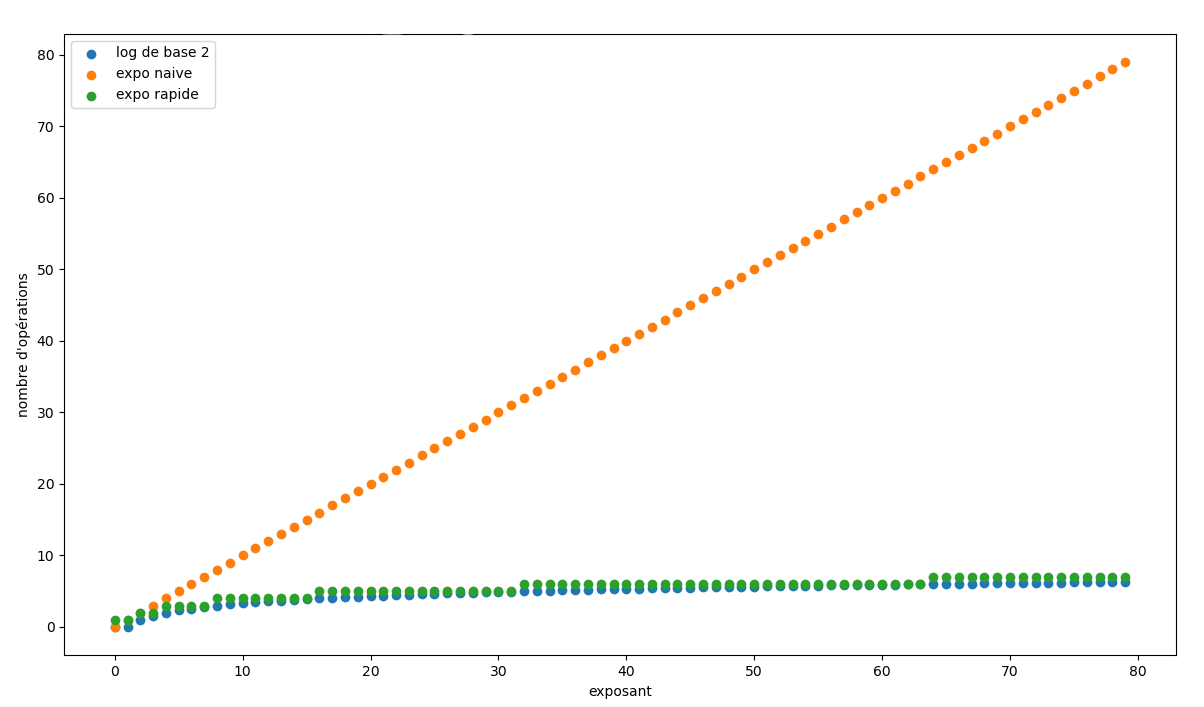
\includegraphics[width=\textwidth]{fig/diff_complexite.png}
    \caption{Comparaison des complexités des deux algorithmes d'exponentiation}
    \label{fig:diff_complexite}
\end{figure}
Il est aussi important de relever que la présence de l'algorithme d’exponentiation rapide n'est pas un hasard, c'est grâce à lui que le système est faillible. En effet, si il rencontre un $1$ dans la représentation binaire du nombre il fait 2 calculs, sinon, s'il rencontre un $0$, il en fait un seul. Grâce à ça, il a une fuite de la clé qui s’opèrera sur la trace de consommation électrique. On gagne en rapidité, mais attention, on fait fuir des données liée à la clé privée ...\\

Une fois ces primitives implémentées, il a été facile d'implémenter la génération de clé, le chiffrement et le déchiffrement, vous pouvez également retrouver ces implémentations en C dans l'archive final du projet.

\subsection{Rapprocher notre implémentation d'un cas d'usage}
A cette étape de l'implémentation du RSA, nous avons un RSA qui fonctionne sur 32 bits, le problème est que cette implémentation est très loin de la réalité.

En effet, d'après les recommandation de l'ANSSI \cite{anssi:guide}, un RSA implémenté avec les types de bases du C ($32$ bits), n'est pas du tout sécurisé. Effectivement, nous pouvons retrouver page 19 les 4 règles suivantes :
\begin{enumerate}
  \item La taille minimale du module est de $2048$ bits, pour une utilisation ne devant
pas dépasser la fin de l’année 2030.
  \item Pour une utilisation à partir de l’année 2031, la taille minimale du module
est de $3072$ bits.
  \item Les exposants secrets doivent être de même taille que le module.
  \item Pour les applications de chiffrement, les exposants publics doivent être strictement supérieurs à $2^{16} = 65536$.
\end{enumerate}
Afin d'attaquer une version du RSA qui pourrait être utilisé dans un cadre réel, nous allons donc devoir l'implémenter avec un module, notée $n$ précédemment, de 2048 bits ! Or, comme vu précédemment nous allons utiliser une machine en 32 bits, ce qui signifie que les types de bases sur lesquels les opérations élémentaires sont implémentées, ne dépasse pas 32 bits. Nous allons devoir créer et implémenter des opérations sur les grands nombres, nous construirons un tableau de plusieurs nombres classique de 32 bits jusqu'à atteindre un nombre de 2048 bits.

\subsection{Implémentation du RSA avec des grands nombres (> 32 bits)}
Pour représenter un grand entier dans un système embarqué 32 bits, nous utilisons un découpage en chunks de 16 bits. Imaginons que nous souhaitons un nombre de 64 bits. Nous divisons cet entier en mots de 16 bits. Ainsi, chaque chunk de 16 bits contient une partie du grand entier.\\

Prenons un exemple concret : supposons que notre grand entier soit \texttt{0xABCD1234567890EF}. Pour le découper en chunks de 16 bits, nous aurons :

\begin{itemize}
\item Chunk 1: \texttt{0xABCD}
\item Chunk 2: \texttt{0x1234}
\item Chunk 3: \texttt{0x5678}
\item Chunk 4: \texttt{0x90EF}
\end{itemize}

Chaque chunk peut être représenté par un entier de 16 bits dans la mémoire du système embarqué. En utilisant cette méthode de découpage, nous pouvons stocker et manipuler des grands entiers même dans des systèmes avec des limitations de taille de données.\\

Si nous utilisons des sous-entiers de 16 bits et pas de 32 bits c'est parce que le 32 bits servira de type d'overflow, en effet lorsqu'on aura une sous opération qui dépassera la taille d'un chunk alors un entier de 32 bits permettra de résoudre ce problème.\\

Sachant que chaque chunk est sur $16$ bits c'est comme si nous avons une représentation du nombre en base $2^{16}$, nous n'avons ``plus'' qu'a considéré un chunk comme un symbole de la base $2^{16}$ et implémenté les opérations usuelles dessus.\\

Cette méthode fonctionne pour l'addition et la soustraction, mais pour les opérations d'inverse modulaire, de multiplication modulaire et de division, cela ne fonctionne plus et il faut utiliser des algorithmes plus poussés, nous nous sommes basé sur ceux du livre ``Handbook of Applied Cryptography'' \cite{hac:ch14}. Nous avons réussi à implémenter les fonctions suivante :
\begin{figure}[H]
\begin{minted}{C}
uint32_t bi_add(bigint_t* out, bigint_t* a, bigint_t* b);
uint32_t bi_mul(bigint_t* out, bigint_t* a, bigint_t* b);
uint32_t bi_sub(bigint_t *res, bigint_t *a, bigint_t *b);
void bi_exp_naif(bigint_t* res, bigint_t* base, uint32_t exp);
void bi_setzero(bigint_t* a);
void bi_mov(bigint_t* src, bigint_t* dst);
void print_bigint(bigint_t *a);
int bi_compare(bigint_t *a, bigint_t *b);
\end{minted}
\caption{Prototypes des fonctions implémentées sur les grands nombres}
\label{fig:proto_fn}
\end{figure}

Le code source des ces fonctions se trouve dans l'archive finale du projet, malheureusement, comme vous pouvez le remarquer, nous n'avons pas réussi à implémenter les opérations de réductions modulaire et sans ça nous ne pouvons pas calculer modulo $n$, mais que faire des calculs sur $\mathbb{Z}$. Nous avons donc été incapable de faire un RSA grandeur nature, mais ce n'est pas non plus très grave car le principe de l'attaque reste le même et toutes les choses que nous avons faites par la suite seront adaptable aisément pour 2048 bits.

\subsection{Conclusion}
Cette section a mis en lumière les différentes étapes de notre implémentation du RSA sur un firmware customisé de la ChipWhisperer. Nous avons débuté en explorant les fondements du RSA sur des nombres de 32 bits, en utilisant les opérations élémentaires disponibles sur la plateforme. Cependant, nous avons rapidement confronté les limites de cette approche lorsque nous avons cherché à nous conformer aux standards de sécurité actuels, nécessitant l'utilisation de clés et de modules de taille beaucoup plus grande. Nous avons donc entrepris d'étendre notre implémentation pour manipuler des nombres de grande taille, en découpant ces nombres en chunks de 16 bits pour surmonter les contraintes de la plateforme. Malgré les progrès réalisés, des défis persistent, notamment dans l'implémentation des opérations de réduction modulaire, qui sont essentielles pour le fonctionnement du RSA à grande échelle. Néanmoins, ces efforts nous ont permis de mieux comprendre les complexités de l'implémentation du RSA dans des environnements embarqués et de poser les bases pour des développements futurs dans ce domaine.